
\chapter{Teoretyczne aspekty projektowania sprzętowych generatorów liczb losowych}

% Rozdział teoretyczny --- przegląd literatury naświetlający stan wiedzy na dany temat. 

% Przegląd literatury naświetlający stan wiedzy na dany temat obejmuje rozdziały pisane na podstawie
% literatury, której wykaz zamieszczany jest w części pracy pt.~\emph{Literatura} (lub inaczej \emph{Bibliografia},
% \emph{Piśmiennictwo}). W tekście pracy muszą wystąpić odwołania do wszystkich pozycji zamieszczonych w
% wykazie literatury. \textbf{Nie należy odnośników do literatury umieszczać w stopce strony.} Student jest
% bezwzględnie zobowiązany do wskazywania źródeł pochodzenia informacji przedstawianych w pracy,
% dotyczy to również rysunków, tabel, fragmentów kodu źródłowego programów itd. Należy także podać
% adresy stron internetowych w przypadku źródeł pochodzących z Internetu.

\noindent Niniejszy rozdział przedstawia teoretyczne podstawy projektoawnia 
sprzętowych generatorów liczb losowych. Omówiona zostanie klasyfikacja architektur generatorów 
oraz fizyczne zjawiska wykorzystywane do pozyskiwania entropii w układach programowalnych 
FPGA. Ponadto wytłumaczne zostaną metody obróbki sygnałów losowych oraz 
standardy statystyczne stosowane do walidacji jakości generowanych danych.

\section{Źródła losowości}



\subsection{TRBG}

\begin{figure}[H]
    \centering
    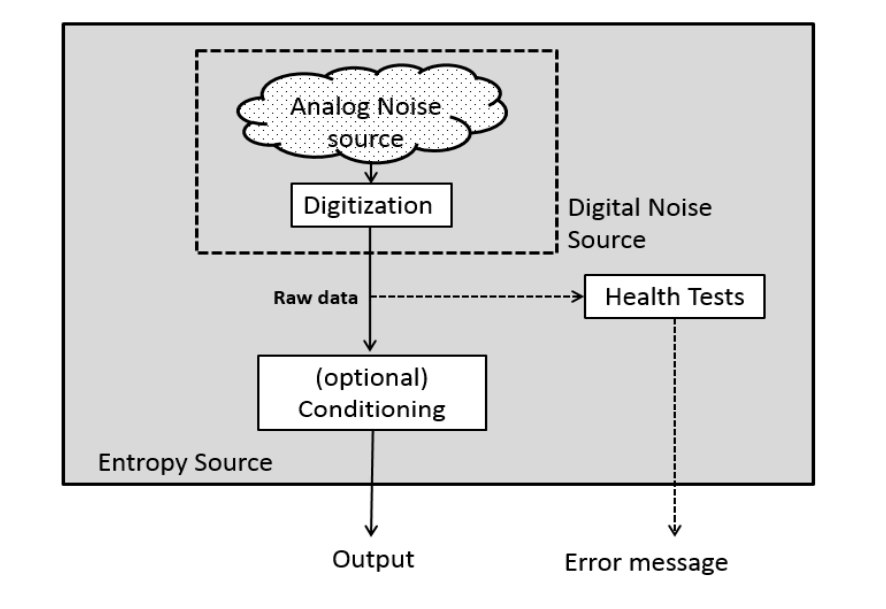
\includegraphics[width=0.75\textwidth]{figures/ch2/nist_source_schematic.png}
    \caption{Model źródła entropii. \cite{NIST-SP-800-90B}}
    \label{fig:ch2_model_zrodla_entropii_nist}
\end{figure}

\subsection{PRBG}

\subsection{QRBG}

\subsection{Zasada działania Quantis USB 4M}

\section{RO jako źródła losowości w FPGA}

\begin{figure}[H]
    \centering
    \includesvg[width=\textwidth]{figures/ch2/schematic.svg}
    \caption{Przykład prostego oscylatora pierścieniowego.}
    \label{fig:ch2_oscylator_3xNOT}
\end{figure}

\section{Ekstraktory losowości}

\subsection{Ekstraktor von Neumanna}

\subsection{Wielomian CRC}

\subsection{Ekstraktor Toeplitz'a}

\subsection{Szyfr strumieniowy AES-CTR}

\section{Metody oceny losowości}

\subsection{ENT - Fourmilab Random Sequence Tester}

\subsection{NIST SP 800-22 - A Statistical Test Suite for Random and Pseudorandom Number Generators for Cryptographic Applications}

\subsection{NIST SP 800-90B - Entropy Assessment Test Suite}

 